\chapter{Isoviscous elastic-plated  gravity current model  for shallow
  magmatic intrusion}

\label{chap2} 
\minitoc

\citet{Michaut:2011kg} proposed  a new  model for  the spreading  of a
shallow   depth   intermediate-size   intrusions,   where   magma   is
continuously injected at the center and is accommodated by the bending
of  the  overlying strata.   In  particular,  the model  differs  from
previous ones by  considering the dynamics of  the emplacement itself,
in a  sense that the  radius in self-consistently determined,  and the
driving  force  associated  with  the magma  weight  which  were  both
neglected   in   older   models.    In   the   original   paper   from
\citet{Michaut:2011kg}, the  model was  derived in both  cartesian and
axisymmetric geometry and the results  were presented in 2D. A similar
model in $2D$ with an additional  fracture criterion at the tip of the
intrusion    has   been    derived   by    \citet{Bunger:2011cb}   and
\citet{Anonymous:QWXp_4JV}  discussed precisely  the  dynamics at  the
contact  line  and  the  case of  an  elastic-plated  gravity  current
spreading over an inclined  plane \citep{Anonymous:QWXp_4JV}.  In this
chapter, we  present a summary  of the model  and the results  for the
spreading of an isoviscous elastic-plated gravity current over a rigid
horizontal  surface in  an axisymmetrical  geometry.  Results  in this
geometry  have been  thoroughly studied  by \citet{Lister:2013ia}  and
this model will constitute the  reference for more elaborate models in
the manuscript.

\section{Model}
\label{C2-sec:model}

The model considers an isoviscous elastic-plated gravity current, i.e.
an  isoviscous  fluid  of  viscosity  $\eta_h$  and  density  $\rho_m$
spreading beneath a thin elastic sheet  of thickness $d_c$ and above a
semi infinite rigid layer \citep{Michaut:2011kg,Bunger:2011cb} (Figure
\ref{C2-Sketch}).  The fluid is injected  continuously at the base and
center of the current at a rate $Q_0$ through a cylindrical conduit of
diameter $a$.

\begin{figure}[htbp]
  \begin{center}
    \graphicspath{ {/Users/thorey/Documents/These/Manuscript/Figure/Chapter2/} }
    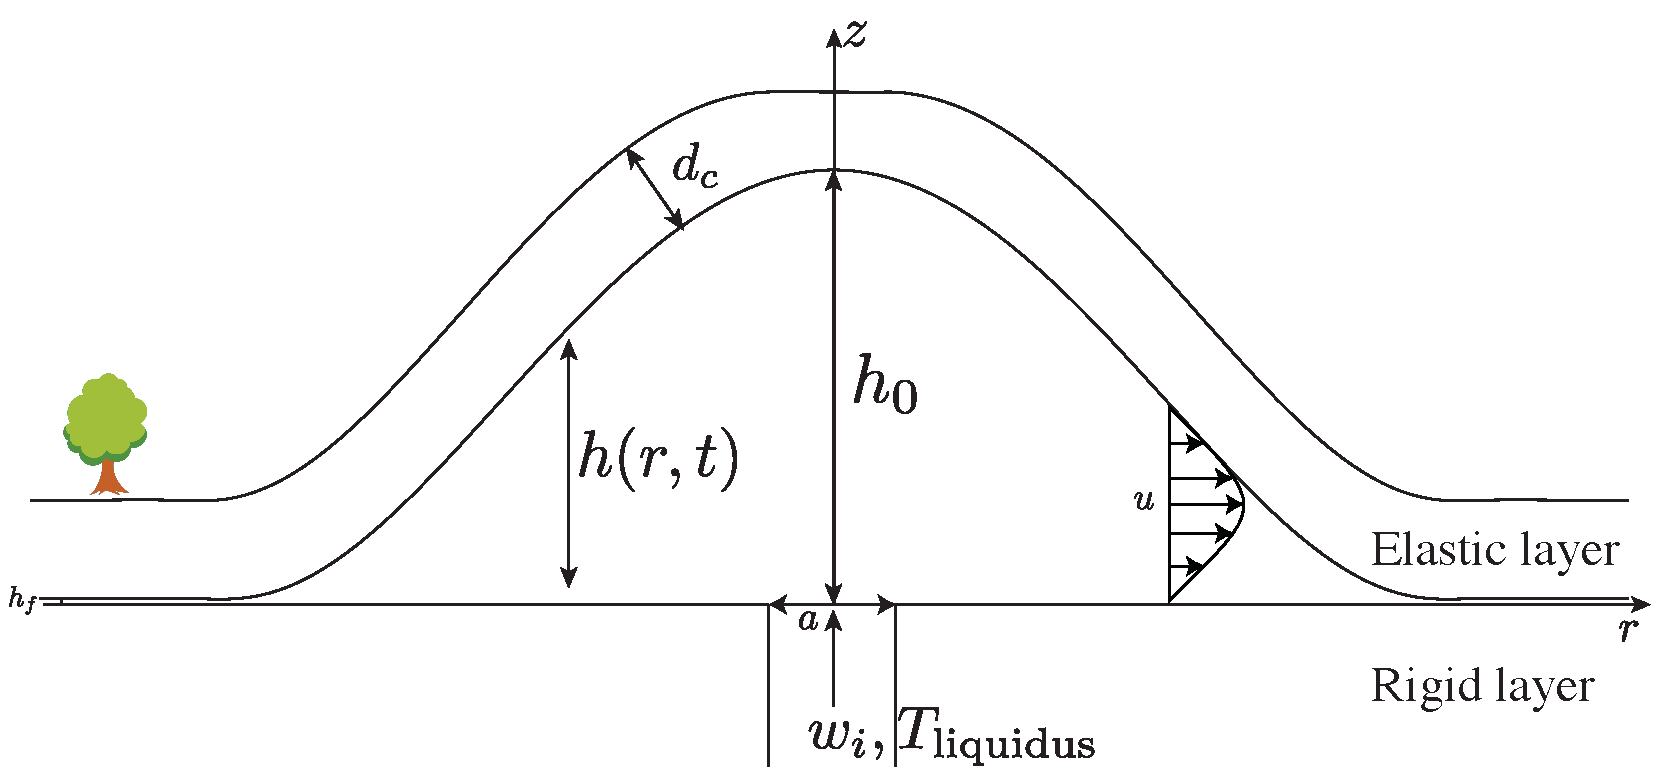
\includegraphics[scale=0.40]{C2_Sketch.pdf}
    \caption{Model geometry and parameters.}
    \label{C2-Sketch}
  \end{center}
\end{figure}

\subsection{Governing equation}
\label{C2-sec:Governing equation}

\textbf{Driving pressure}\\

The  intrusion develops  over a  length scale  $\Lambda$ that  is much
larger than its  thickness $H$ ($\epsilon = H/ \Lambda<<  1$).  In the
laminar  regime  and  in  axisymmetrical  coordinates  ($r$,$z$),  the
Navier-stokes equations within the lubrication assumption are
\begin{eqnarray}
  -\frac{\partial P}{\partial r}  +  \frac{\partial}{\partial z}\left(\eta \frac{\partial u}{\partial z}\right) &=&0\label{C2_V1} \\
  -\frac{\partial P}{\partial z}  - \rho_{m}g&  =&0\label{C2-Npressure}
\end{eqnarray}
where  $u(r,z,t)$  is  the  radial   velocity,  $g$  is  the  standard
acceleration due to gravity and  $P(r,z,t)$ is the pressure within the
fluid.   Integration  of  (\ref{C2-Npressure}) thus  gives  the  total
pressure  $P(r,z,t)$ within  the flow.   When the  vertical deflection
deflection $h(r,t)$  of the upper  elastic layer is small  compared to
its thickness  $d_c$, i.e $h<<d_c$,  we can neglect stretching  of the
upper layer and only consider  bending stresses.  Therefore, the total
pressure $P(r,z,t)$ at a level $z$ in the intrusion is the sum of four
contributions: the  weight of the  magma and  of the upper  layer, the
bending pressure $P_b$ and the atmospheric pressure $P_0$
\begin{equation}
  P = \rho_m g (h-z)+\rho_rgd_c+P_b+P_0
  \label{C2-pression}
\end{equation}
where $h(r,t)$ is the intrusion  thickness and $\rho_r$ the density of
the surrounding rocks. The bending pressure  is given by the force per
unit area  that is necessary  for a  vertical displacement $h$  of the
thin elastic plate \citep{Turcotte:1982ca}
\begin{equation}
  P_d = D\nabla^4h
\end{equation}
where $D$  is the flexural  rigidity of  the thin elastic  layer, that
depends on the Young's modulus $E$, Poisson's ratio $\nu^*$ and on the
elastic           layer          thickness           $d_c$          as
$D = Ed_c^3/\left(12(1-\nu^*)\right)$.

\vspace{.5cm} \textbf{Velocity field} \vspace{.5cm}

At the contact with the elastic sheet $z=h(r,t)$, the no-slip boundary
condition is present  and so, the tangential velocity is  zero and the
normal velocity  is the change  in height ($\partial h/  \partial t$).
With $\vec{n}$ the normal to the surface and $\vec{t}$ the tangent, we
have
\begin{eqnarray}
  \vec{n} \cdot (u,w) &=& \frac{\partial h }{\partial t}\\
  \vec{t} \cdot (u,w) &=& 0 \label{tangeant}.
\end{eqnarray}
The  tangent  vector is  $\vec{t}  =  (1,  \partial h/  \partial  r)$.
However, within the lubrication  assumption, the vertical component of
the  tangent  vector scales  as  $\epsilon$  and thus,  is  negligible
compared to  the radial  component. Therefore, the  boundary condition
($\ref{tangeant}$) reduces  to $u(r,z=h,t)  =0$.  At  the base  of the
flow, the same boundary condition hold and $u(r,z=0,t) =0$.

Equation (\ref{C2_V1}) is integrated twice  as a function of $z$ using
these boundary conditions and the horizontal velocity is
\begin{equation}
  u(r,z,t) =\frac{1}{2\eta} \frac{\partial P}{\partial r} \left(z^2-hz\right)
  \label{C2-vel}
\end{equation}

\vspace{.5cm} \textbf{Injection rate} \vspace{.5cm}

The effective overpressure $\Delta P^*$ driving the flow in the feeder
conduit decreases as the intrusion thickens and is given by
\begin{equation}
  \Delta P^* = \Delta P -\rho_m g h_0 \label{C2-Q0}
\end{equation}
where $h_0(t)$ is the maximum  intrusion thickness at the center $r=0$
and $\Delta P$ is the initial  driving pressure or the overpressure at
the base of the dyke ($z = -Z_c$).

In (\ref{C2-Q0}), the bending pressure  at then center, which scale as
D$h_0(t)/R(t)^4$  where  $R(t)$  is   the  blister  radius,  has  been
neglected.  Although  it tends  to infinity at  the initiation  of the
flow, it rapidly  vanishes as the blister spreads  and the hydrostatic
pressure $\rho_m g h_0$ becomes  the main contribution to the pressure
at the  center.  In addition, the  model assumes a large  aspect ratio
for the blister and does not consider the initiation of the flow.

Finally,  assuming a  Poiseuille flow  within the  cylindrical feeding
conduit, the vertical injection velocity $w_i(r,t)$ and injection rate
$Q(t)$ are given by
\begin{equation}
  w_i=
  \begin{cases}
    \frac{ \Delta P^*}{4 \mu Z_{c}} (\frac{a^{2}}{4}-r^{2})& r \le \frac{a}{2}\\
    0 & r > \frac{a}{2}
  \end{cases}
  \label{C2-eq12}
\end{equation}
\begin{equation}
  Q = Q_0(1-\frac{\rho_m g h_0}{\Delta P})
  \label{C2-eq11}
\end{equation}
where
$Q_0=\left(\pi \Delta P^* a^{4}\right)/\left(128 \eta Z_c\right)$.

\vspace{.5cm} \textbf{Mass conservation} \vspace{.5cm}

The fluid  is assumed  incompressible and a  global statement  of mass
conservation gives
\begin{eqnarray}
  \frac{\partial         h}{\partial        t} +\frac{1}{r}
  \frac{\partial}{\partial
  r} \left( r\int_0^hudz\right) = w_i
  \label{C2-Mass}
\end{eqnarray}
and using (\ref{C2-vel}), we find  that the equation for the evolution
of the thickness in time and space reads
\begin{equation}
  \frac{\partial h}{\partial t} =\frac{\rho_mg}{12 \eta r}
  \frac{\partial}{\partial r}  \left( rh^3  \frac{\partial h}{\partial
      r}\right)+\frac{D}{12\eta r} \left( rh^3 \frac{\partial}{\partial r}\nabla^4h\right)+
  w_i .\label{C2-Heq}
\end{equation}
It is  composed of three different  terms on the right  hand side. The
first term represents gravitational  spreading, i.e.  spreading of the
blister under its own weight. The second term represents the squeezing
of the  flow by the upper  elastic layer.  Both term  are negative and
induces spreading.   The last term  represents fluid injection  and is
positive.

\subsection{Dimensionless equations}
\label{C2-sec:dimens-equat}

Equations  (\ref{C2-eq12}) and  (\ref{C2-Heq}) are  nondimensionalized
using a  horizontal scale $\Lambda$, a  vertical scale $H$ and  a time
scale $\tau$ given by
\begin{eqnarray}
  \Lambda &=& \left(\frac{D}{\rho_m g}\right)^{1/4}\label{L1}\\
  H&=&\left       (\frac{12\eta      Q_{0}}{\rho_{m}g       \pi}\right      )
       ^{\frac{1}{4}} \label{H1}\\
  \tau&=&\frac{\pi \Lambda^{2} H}{Q_{0}}\label{T1}
\end{eqnarray}

where scales  are chosen  such that $Q_0  = \pi\Lambda^2  H/\tau$. The
length scale $\Lamba$ represents the  flexural wavelength of the upper
elastic layer,  i.e. the  length scale at  which bending  stresses and
gravity  contributes equally  to flow.   The height  scale $H$  is the
thickness of  a typical gravity current  and the time scale  $\tau$ is
the  characteristic time  to  fill  up a  cylindrical  flow of  radius
$\Lambda$ and thickness  $H$ at constant rate $Q_0$.   In addition, we
can       define        a       horizontal        velocity       scale
$U=\Lambda/\tau=\left(\rho_m           g           H^3\right)/\left(12
  \eta_h\Lambda\right)$.

The dimensionless equation is
\begin{eqnarray}
  \frac{\partial h}{\partial t}& =&\frac{1}{ r}
                                    \frac{\partial}{\partial r}  \left( rh^3  \frac{\partial h}{\partial
                                    r}\right)+\frac{1}{ r} \left( rh^3
                                    \frac{\partial}{\partial
                                    r}\nabla^4h\right)\nonumber\\
                               &+&
                                   \frac{32}{\gamma^{2}}\left(\frac{1}{4}-\frac{r^{2}}{\gamma^{2}}\right)\left(1-\frac{h_0}{\sigma}\right)
                                   \label{C2-mainEq}
\end{eqnarray}
where the last term is replaced by zero for $r>\gamma/2$. $\gamma$ and
$\sigma$ are  two dimensionless numbers  that control the  dynamics of
the flow
\begin{eqnarray}
  \gamma &=& \frac{a}{\Lambda}\\
  \sigma &=& \frac{\Delta P}{\rho_m g h}.
\end{eqnarray}
$\gamma$  is the  dimensionless radius  of  the conduit,  it does  not
significantly influence the flow and is set to $0.02$ in the following
\citep{Michaut:2009jx,Michaut:2011kg}.   $\sigma$  is  the  normalized
pressure  head,  i.e.,  the  ratio between  the  initial  overpressure
driving the flow and the weight of the magma at the center.
	 
\subsection{Need for regularization}
\label{C2-sec:need-regularization}

One  of   the  main   mathematical  difficulty  in   solving  equation
(\ref{C2-mainEq}) arises at the  contact line.  Indeed, the assumption
that the  thickness of  the fluid  tends to zero  at the  contact line
leads       to       divergent      viscous       stresses,       i.e.
$\eta  \partial   u/\partial  z\rightarrow  \infty$  and   hence,  the
theoretical         immobility          of         the         blister
\citep{Flitton:1999iv,Lister:2013ia,Anonymous:QWXp_4JV}. This problem,
known  a  the  contact-line  paradox,  is  a  well  know  problem  for
surface-tension driven flow  such as the spreading of  a water droplet
\citep{Bertozzi:1998wz,Snoeijer:2013cm}.

The formal proof  have been derived by  \citet{Flitton:1999iv} and can
be derived  as follow. Suppose  that (\ref{C2-mainEq}) has  a solution
and the solution has the  form $h \sim A(t)(R(t)-r)^{\alpha}$ near the
contact line.  As $r \rightarrow R(r)$, the bending term dominates the
gravitational term and (\ref{C2-mainEq}) reduces to
\begin{eqnarray}
  \frac{\partial       h}{\partial       t}&      =&\frac{1}{       r}
                                                     \frac{\partial}{\partial r}\left( rh^3 \frac{\partial}{\partial r}\nabla^4h\right).
                                                     \label{C2-mainEq2}
\end{eqnarray}
Injecting the  solution into  (\ref{C2-mainEq2}) and keeping  only the
leading powers of $R-r$ gives
\begin{eqnarray}
  \frac{\partial    R}{\partial    t}    A\alpha\left(R-r\right)^{\alpha-1}+
  \frac{\partial           A}{\partial           t}\left(R-r)^{\alpha}
  &=&A^4\alpha(\alpha-1)(\alpha-2)\nonumber\\
  &&(\alpha-3)(\alpha-4)(\alpha-5)(R-r)^{4\alpha-6}\nonumber
\end{eqnarray}
The time derivative is locally dominated by its convective part at the
tip, the second  term on the left  is small compared to  the first and
therefore,   by   equating   the   exponent  of   $R-r$,   we   obtain
$\alpha = 5/3$, and by equating the coefficients, we deduce
\begin{equation}
  \frac{\partial R}{\partial r} =-\frac{280}{243} A^3.
\end{equation}
It shows that (\ref{C2-mainEq}) can  only have retreating contact line
($dR/dt<0$)   but  not   with  advancing   contact  line   ($dR/dt>0$)
\citep{Lister:2013ia,Flitton:1999iv}.

To  mitigate this  problem,  one  common approach  is  to  add a  thin
prewetting film, with thickness $h_f$ such that $h\rightarrow h_f$ as
$r\rightarrow  \infty$.   While  the  solution will  depend  upon  the
prewetting  film thickness  $h_f$ and  will not  show any  convergence
properties when $h_f\rightarrow 0$, we will see that the dependence in
$h_f$ is  weak and the  difference between different values  for $h_f$
will  be  relatively  small  \citep{Lister:2013ia,Anonymous:QWXp_4JV}.
Unless otherwise specified, we will consider $h_f = 5\cdot 10^{-3}$ in
the manuscript.



\section{Results}
\label{C2-sec:regime-propagations}

For  a  small  prewetting   film  thickness,  i.e.   $h_f/H<<1$,  the
numerical  resolution of  the  equation  (\ref{EqFinal1}) shows  three
spreading regimes:  a bending  regime where  gravity is  negligible, a
viscous  gravity current  regime  where bending  is  negligible and  a
regime               of              lateral               propagation
\citep{Michaut:2011kg,Bunger:2011cb,Lister:2013ia}.

\begin{figure}[h!]
  \begin{center}
    \graphicspath{ {/Users/thorey/Documents/These/Manuscript/Figure/Chapter2/} }
    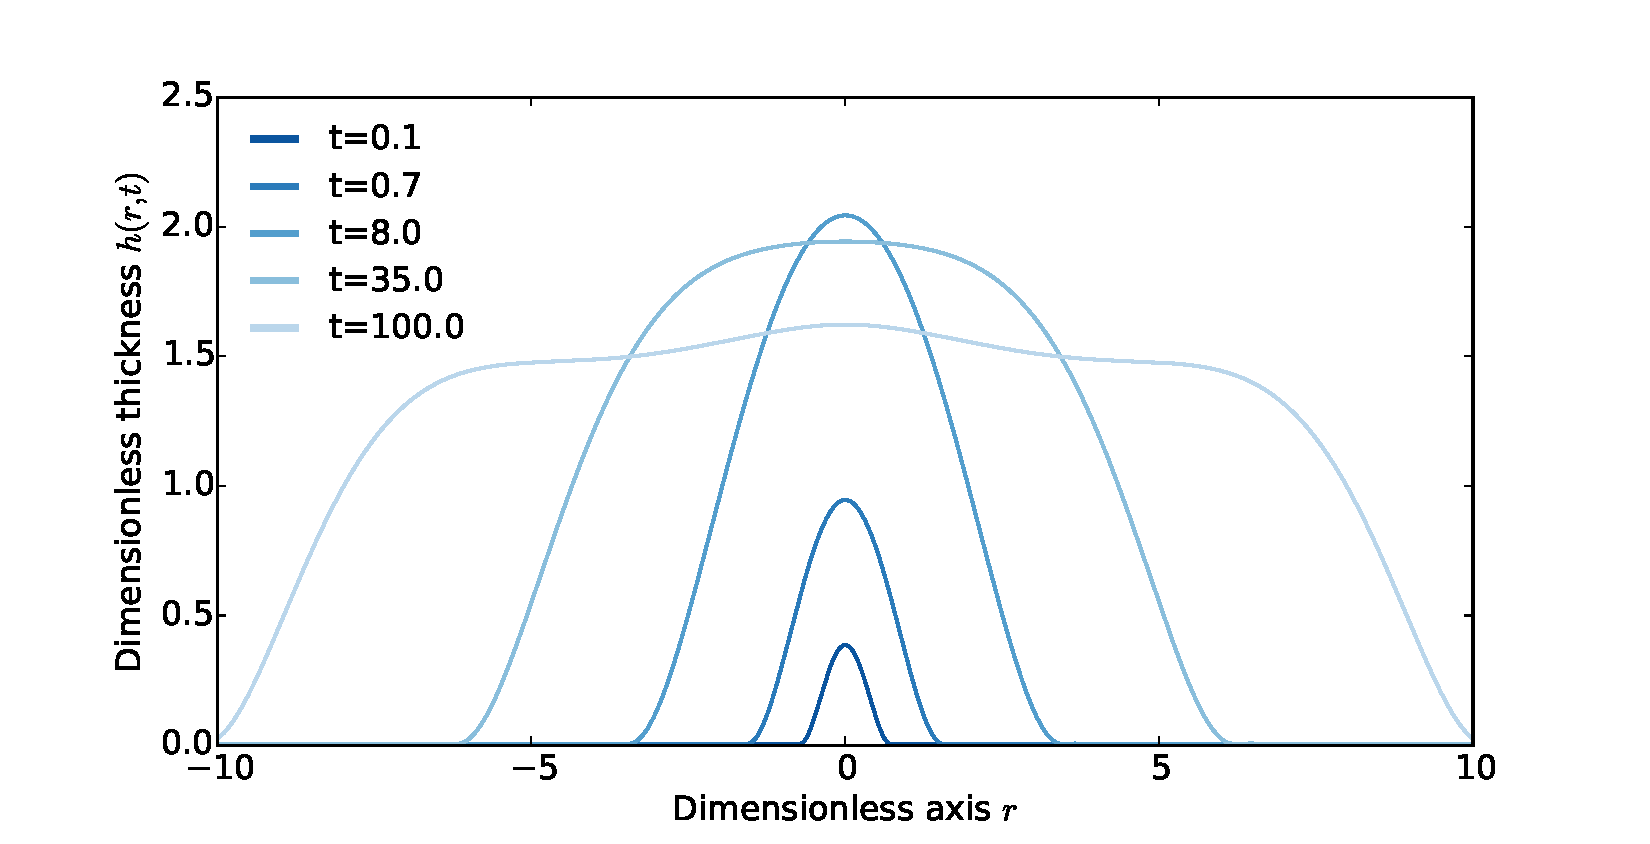
\includegraphics[scale=0.5]{C2_ELAS_GRAV_Profil.eps}
    \caption{Shape of the flow, i.e.  thickness $h(r,t)$ as a function
      of the radial axis $r$ at  five different times indicated on the
      plot. Variables are  dimensionless and one needs  to multiply by
      the characteristic  scales (thickness,  length or time  given by
      (\ref{H1}),  (\ref{L1})  or  (\ref{T1})) to  obtain  dimensional
      values.   For $t<10$,  the intrusion  is in  the bending  regime
      whereas  for $t>10$  the  intrusion is  in  the gravity  current
      regime.}
    \label{C2_ELAS_GRAV_Profil}
  \end{center}
\end{figure}

\subsection{Bending regime}
\label{C2-sec:bending-regime}

At  early times,  when  $R<<\Lambda$, gravity  is  negligible and  the
dynamics of  the spreading  is governed  by the  bending of  the upper
layer.   In addition,  if $h_0<<\sigma$,  the overpressure  $\Delta P$
driving the flow is much larger than  the weight of the blister at the
center and the injection rate can be considered constant.

In that case, the spreading is  very slow and the interior has uniform
pressure $P =\nabla^4h$.  The flow is bell-shaped and its thickness is
given by
\begin{equation}
  h(r,t) = h_0(t)\left(1-\frac{r^2}{R^2(t)}\right)^2
  \label{IntrusionShape}
\end{equation}
with  $h_0(t)$   the  thickness  of   the  intrusion  at   the  center
\citep{Michaut:2011kg,Lister:2013ia}.       In       this      regime,
\citet{Lister:2013ia} have  shown that the spreading  is controlled by
the propagation  of a peeling by  bending wave at the  intrusion front
with dimensionless velocity $c$
\begin{equation}
  c=    \frac{\partial             R}{\partial            t}             =h_f^{1/2}
  \left(\frac{\kappa}{1.35}\right)^{5/2}
  \label{WaveVelocity}
\end{equation}
where  $\kappa  =  \partial^2  h/\partial r^2$  is  the  dimensionless
curvature  of  the  interior  solution.   Using  the  propagation  law
(\ref{WaveVelocity})   and  the   form   of   the  interior   solution
(\ref{IntrusionShape}), they  find that the  radius and the  height of
the intrusion are given by similarity solutions
\begin{eqnarray}
  R(t) &=& 2.2h_f^{1/22}t^{7/22}\label{ScalingR}\\
  h_0(t)&=&0.7 h_f^{-1/11}t^{8/22}\label{ScalingH}.
\end{eqnarray}
where the numerical pre-factor have been matched to our simulations.

\begin{figure}
  \begin{center}
    \graphicspath{ {/Users/thorey/Documents/These/Manuscript/Figure/Chapter2/} }
    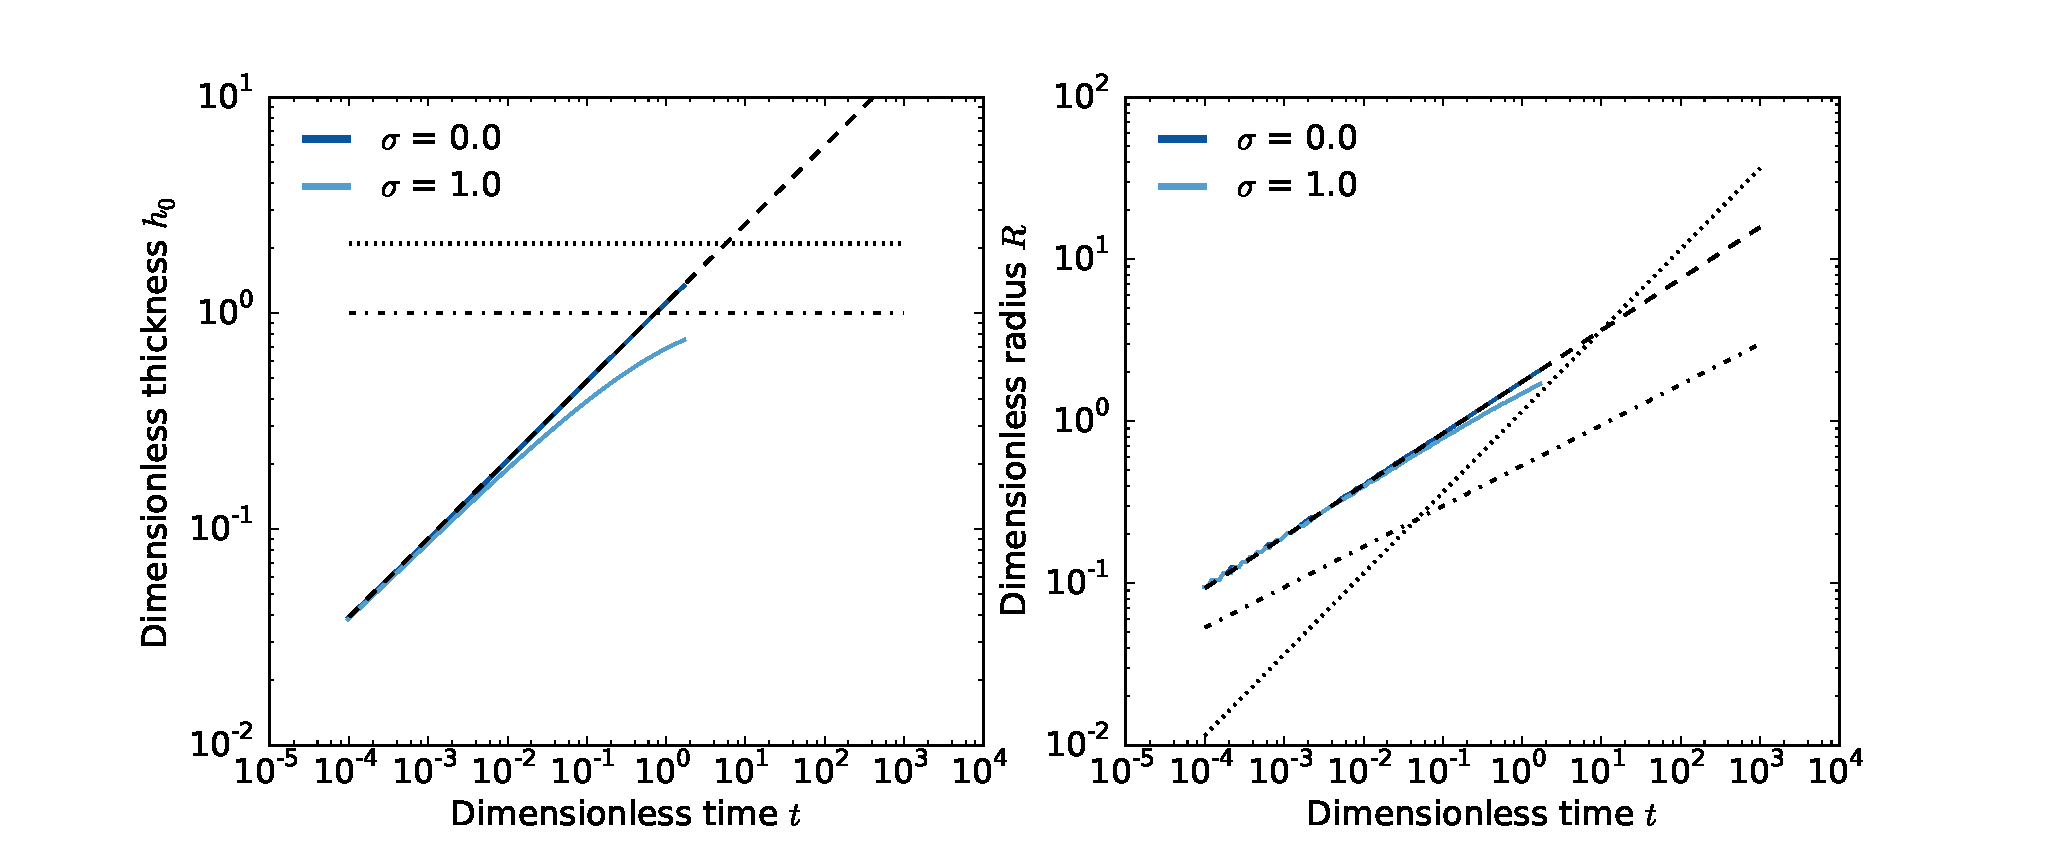
\includegraphics[scale=0.4]{C2_ELAS_GRAV_Sigma.eps}
    \caption{Left: Dimensionless thickness at  the center $h_0$ versus
      dimensionless  time  $t$   for  different  dimensionless  number
      $\sigma$  indicated on  the  plot.   Dashed-lines represent  the
      scaling  laws in  the different  regimes.  Right:  Dimensionless
      radius  $R$   versus  dimensionless   time  $t$  for   the  same
      dimensionless  number  $\sigma$.    Dashed-lines  represent  the
      scaling laws in the different regimes.}
    \label{C2_ELAS_GRAV_Sigma}
  \end{center}
\end{figure}

\subsection{Gravity current regime}
\label{C2-sec:grav-curr-regime}

In  contrast, when  the radius  R becomes  much larger  than $\Lambda$
($R>>\Lambda$), the weight of the  intrusion becomes dominant over the
bending  terms.  The  pressure is  given by  the hydrostatic  pressure
$P = h$  and the intrusion enters a classical  viscous gravity current
regime where bending terms only affect the solution near the intrusion
edge   \citep{Huppert:1982a,Michaut:2011kg,Lister:2013ia}.   In   this
second regime, the radius evolves as $t^{1/2}$ and the thickness tends
to a constant
\begin{eqnarray}
  R(t) &=& 0.715 t^{1/2}\label{Scaling-R-Gravi}\\
  h_0 &=& 1.86\label{Scaling-H-Gravi}
\end{eqnarray} 

\subsection{Lateral propagation}
\label{sec:lateral-propagation}

Once $h_0\rightarrow \sigma$,  the flow is thick  enough to compensate
for  the initial  overpressure. The  thickness at  the center  remains
constant and  the flow enters  a regime of lateral  propagation, where
only its radius $R(t)$ is  to increase \citep{Michaut:2011kg}. In this
regime, except at the center when it redistributes the pressure over a
length scale $\Lambda$, the bending term is negligible compared to the
gravitational  term. \citet{Michaut:2011kg}  has  shown  that in  this
regime, the thickness is constant and the radius evolves as $t^{1/4}$
\begin{eqnarray}
  R(t) &=& \left(\frac{\sigma^3 t}{4\pi}\right)^{1/4}\label{Scaling-R-Propa}\\
  h_0 &=& \sigma\label{Scaling-H-Propa}
\end{eqnarray} 

\section{Application to laccoliths}
\label{C2-sec:appl-earth-moon}

\subsection{Range of value for the parameters}
\label{sec:range-value-param}

In terrestrial settings,  lava density $\rho_m$ depends  mainly on its
composition and varies between $ 2300$ kg m$^{-3}$ for felsic lavas to
$3000$ kg m$^{-3}$ for mafic  lavas. Hence, for Young's modulus values
between $10$ and $100$ GPa and  intrusion depths between $0.1$ and $5$
km, the characteristic  length scale $\Lambda$ varies  between $1$ and
$10$  km.   The overpressure  in  magma  reservoirs driving  dykes  is
typically    between    a    few    to    several    tens    of    MPa
\citep{Tait:1988vn,Marti:2000fe} and  the conduit length  $Z_c$ varies
from a few  to several tens of kilometers. Lava  viscosity at eruption
temperature  $\eta_h$  depends mainly  on  its  composition and  water
content; close to its liquidus temperature,  it can varies from $1$ Pa
s  for   ultramafic  lavas   to  $10^{6}$  Pa   s  for   felsic  lavas
\citep{Anonymous:CZVBrBvv,Giordano:2008em,Whittington:2009fv,Chevrel:2013jn}.
Hence,  injection  rate  $Q_0$  are in  a  range  $10^{-3}-0.1$  m$^3$
s$^{-1}$ and  the height scale  $H$ varies  between $0.1$ m  for mafic
lavas to  $1$ m for  felsic lavas.   Therefore, the time  scale $\tau$
varies  from a  few months  for mafic  lavas to  few years  for felsic
lavas.

\begin{figure}
  \begin{center}
    \graphicspath{ {/Users/teihorey/Documents/These/Manuscript/Figure/Chapter2/} }
    \includegraphics[scale=0.35]{C2_Geological_Data.eps}
    \caption{}
    \label{C2_Geological_Data}
  \end{center}
\end{figure}

\subsection{Earth : Observation Vs Prediction}
\label{sec:observ-vs-pred}

\vspace{.5cm} \textbf{Dataset} \vspace{.5cm}

\citet{E:2015tl} have  made an  extensive catalog of  $900$ laccoliths
across  the  world.   In   particular,  \citet{E:2015tl}  provide  the
thickness and  the radius  of $168$ laccoliths  among which,  $40$ are
also  provided  with  an  estimation  of  the  intrusion  depth.   The
thickness  ranges from  $100$  meters  to $10$  km  and, although  the
largest one goes up to $100$ km, their radius mostly range form $1$ to
$10$  km.  While  most of  the data  are located  in the  United State
($\sim 90\%$), the different laccoliths are widely spread among on the
territory and variation in the parameters between different laccoliths
is most  likely to be  important. Therefore,  in addition to  the data
from  \citet{E:2015tl},  we  also  consider in  this  study  the  data
provided by \citet{Rocchi:2002jy} on $9$ laccoliths nested in the same
christmas tree structure. For this  dataset, each laccolith is part of
a  larger  intrusive  system,  and  hence  variability  of  the  model
parameters should be  limited, except for the  overlying elastic layer
thickness, taken  to be the  intrusion depth, whose  variation between
laccoliths is  given by \citet{Rocchi:2002jy}. Indeed,  the dispersion
is much smaller  for this dataset, the radius ranges  from $1$ to $10$
km and the thickness from $40$m to $1$ km. In order to account for the
intrinsic scale of different settings for each intrusion, the data are
first   nondimensionalized  using   characteristic   values  for   the
parameters and the intrusion depth, when known, for the data.

\begin{figure}
  \begin{center}
    \graphicspath{ {/Users/thorey/Documents/These/Projet/Refroidissement/Skin_Model/Figure/Figure_Data/} }
    \includegraphics[scale=0.42]{Corry_Rocchie.eps}
    \caption{Left: Thickness $h_0$  (m) versus the radius  $R$ (m) for
      laccoliths   reported   by    \citet{E:2015tl}   in   blue   and
      \citet{Rocchi:2002jy} in red.  Right: Dimensionless thickness as
      a  function of  dimensionless radius,  characteristic thickness,
      and  length  are  calculated  from  (\ref{H1})  and  (\ref{L1}).
      Dashed lines: predicted scaling law from the simulations (black)
      and  best fit  for the  power  law $h_0=aR^b$  for each  dataset
      obtained from a linear least-square regression in log-log space.
      I  use  for the  parameters,  $g=9.81$  m s$^{-2}$,  $Q_0=  0.1$
      m$^{3}$  s$^{-1}$, $\rho_m=2500$  kg  m$^{-3}$,  $E=10$ GPa  and
      $\eta_h=10^6$ Pa s.  Unless the intrusion depth is  given by the
      dataset, we use $d_c=1500$ m and $\nu^*=0.25$.}
    \label{Corry_Rocchie}
  \end{center}
\end{figure}



\vspace{.5cm} \textbf{Range of value for the parameters} \vspace{.5cm}

In terrestrial settings,  lava density $\rho_m$ depends  mainly on its
composition and varies between $ 2300$ kg m$^{-3}$ for felsic lavas to
$3000$ kg m$^{-3}$ for mafic  lavas. Hence, for Young's modulus values
between $10$ and $100$ GPa and  intrusion depths between $0.1$ and $5$
km, the characteristic  length scale $\Lambda$ varies  between $1$ and
$10$  km.   The overpressure  in  magma  reservoirs driving  dykes  is
typically    between    a    few    to    several    tens    of    MPa
\citep{Tait:1988vn,Marti:2000fe} and  the conduit length  $Z_c$ varies
from a few  to several tens of kilometers. Lava  viscosity at eruption
temperature  $\eta_h$  depends mainly  on  its  composition and  water
content; close to its liquidus temperature,  it can varies from $1$ Pa
s  for   ultramafic  lavas   to  $10^{5}$  Pa   s  for   felsic  lavas
\citep{Anonymous:CZVBrBvv,Giordano:2008em,Whittington:2009fv,Chevrel:2013jn}.
Hence,  injection  rate  $Q_0$  are in  a  range  $10^{-3}-0.1$  m$^3$
s$^{-1}$ and  the height scale  $H$ varies  between $0.1$ m  for mafic
lavas to  $1$ m for  felsic lavas.   Therefore, the time  scale $\tau$
varies  from a  few months  for mafic  lavas to  few years  for felsic
lavas.

The model  also considers  a thin pre-wetted  film of  thickness $h_f$
whose  meaning in  the application  to the  spreading of  laccolith is
unclear.  In  particular, the  model shows  no convergence  when $h_f$
tends to zero \citep{Lister:2013ia} and therefore, the thickness $h_f$
might be  linked to some structural  length scale at the  front of the
laccolith or  to the natural  imperfection of the flow  geometry.  For
the purpose of the application, we  choose a film thickness of $1$ mm,
i.e.  the  minimum length  scale with  physical signification  for the
spreading of laccoliths  which give a dimensionless  $h_f$ that varies
between $10^{-2}$ and $10^{-4}$.  The limited effect of changing $h_f$
is detailed in  Appendix \ref{FilmThickness} and in  the following, we
set $h_f$ to $10^{-3}$.

\vspace{.5cm} \textbf{Comparison with the model} \vspace{.5cm}

Using these depths and characteristic values for various properties of
the system, the length and thickness  scales can be estimated for each
laccolith  such   that  the   data  can  be   nondimensionalized.   To
characterize  the mean  trend in  each population,  we make  use of  a
linear least-square regression in log-log  space to obtain a power law
relationship  of the  form $h_0=aR^b$  as predicted  by the  model and
\citet{McCaffrey:1997ea}.  We found $h_0=170 R^{0.63\pm 0.08}$ for the
laccolith of Corry and $h_0=135 R^{1.21\pm 0.1}$ for the laccoliths at
Elba Island.

The model evolution of the radius $R$  of the current as a function of
its thickness can be easily derived from thickness $h_0$ as a function
of its radius $R$ for a current  that solidifies in the third phase of
the   bending  regime   can   be  derived   from   the  scaling   laws
(\ref{ScalingH}) and (\ref{ScalingR}) and should follow
\begin{equation}
  h_0 \sim 0.75 R^{8/7}\label{Hr}
\end{equation}

For the laccolith  system at Elbas Island, the  best fit dimensionless
thickness  for  $h_0$ is  proportional  to  $R^{1.21}$, a  little  bit
smaller than  the model  prediction. \citep{Michaut:2011kg}  founds in
$2D$ that  $R^{1.25}$, The  geometry of these  laccoliths is  not well
known  and probably  not  perfectly two‐dimensional  or circular,  the
value nicely insert between the  two. The dimensionless radius is also
smaller   than   $4$   supporting   their  arrest   in   the   bending
regime. However, the model prefactor is not explain b

\section{Discussion}
\label{C2-sec:discussion}

\begin{table}
  \caption{Range of values for the model parameters}
  \centering
  \begin{tabular}{c|c|c|c|c}
    Parameters& Symbol & Earth & Moon&Unit\\
    \hline
    &&&&\\
    Depth of intrusion & $d_c$ & $0.1-5$ &$0.1-5$ &km \\
    Young's Modulus & $E$ & $10-100$ &$10-100$ &GPa \\
    Poisson's ratio & $\nu^*$ & $0.25$ &$0.25$ &\\
    Gravity & $g$ & $9.81$ &1.62&m s$^{-2}$ \\
    Crust density & $\rho_{r}$ & $2500$ &$2500$&kg m$^{-3}$ \\
    Magma density & $\rho_{m}$ & $2500-3000$ &$3000$&kg m$^{-3}$ \\
    Magma viscosity & $\eta_h $ & $1-10^{4}$ &$1-10^{2}$&Pa s \\
    Feeder dyke width & $a$ & $1-100$ &$1-10$&m \\
    Depth of the melt source & $Z_{c}$ & $ 1-10$&$200-500$& km \\ 
    Initial overpressure & $\Delta P$ & $5-50$ &$1-5$ &MPa \\
    Injection rate & $Q_{0}$ &$0.01-1$ &$1-10$&m$^{3}$ s$^{-1}$ \\
              &&&&\\
    \hline
    Characteristic scales & Symbol & Range of values & Unit\\
    \hline
              &&&&\\
    Height scale & $H$& $0.1-10$ &$0.1-1$ &m \\
    Length scale & $\Lambda$ & $1-12$&$1-20$& km \\
    Time scale & $\tau$ & $10^{-1}-10$&$10^{-2}-1$& years \\
    \label{tab2}
  \end{tabular} 
\end{table}


\begin{table}
  \caption{Range of values for the model parameters}
  \centering
  \begin{tabular}{c|c|c|c}
    \hline
    Parameters& Symbol & Range of values &Unit\\
    \hline
              &&\\
    Depth of intrusion & $d_c$ & $0.1-5$ &km \\
    Young's Modulus & $E$ & $10-100$ &GPa \\
    Poisson's ratio & $\nu^*$ & $0.25$ &\\
    Gravity & $g$ & $9.81$ &m s$^{-2}$ \\
    Magma density & $\rho_{m}$ & $2800-3200$ &kg m$^{-3}$ \\
    Magma viscosity & $\eta $ & $1-10^{4}$ &Pa s \\
    Feeder dyke width & $a$ & $1-100$ &m \\
    Depth of the melt source & $Z_{c}$ & $ 5-500$& km \\ 
    Initial overpressure & $\Delta P$ & $5-50$ &MPa \\
    Injection rate & $Q_{0}$ &$10p{-3}-0.1$ &m$^{3}$ s$^{-1}$ \\
    Crust density & $\rho_{r}$ & $2500$ &kg m$^{-3}$ \\
              &&\\
    \hline
    Characteristic scales & Symbol & Range of values & Unit\\
    \hline
              &&\\
    Height scale & $H$& $0.1-10$ &m \\
    Length scale & $\Lambda$ & $1-12$& km \\
    Time scale & $\tau$ & $10^{-1}-10$ &years \\
    \label{tab2}
  \end{tabular} 
\end{table}


\bibliographystyle{agufull08}
\bibliography{/Users/thorey/Dropbox/Library}



%%% Local Variables:
%%% mode: latex
%%% TeX-master: "../main"
%%% End:
